\chapter{Image Sentiment Analysis}

\section{Introduction}

In~\cite{battiato2016social} we presented \textit{The Social Picture}, a framework to collect and explore huge amount of crowdsourced social images about public events, cultural heritage sites and other customized private events. %which invove the creation of a ``flow of social pictures''.
Through \textit{The Social Picture} users contributes to the creation of image collections about common interests. %Users can add an image to a collection by using either a mobile application and a website interface. Furthermore, an event collection can be populated by selecting images from the most common social networks for images (e.g., Flickr, Panoramio, Instagram).
The collections can be explored through a number of advanced Computer Vision and Machine Learning algorithms, able to capture the visual content of images in order to organize them in a semantic way. The interfaces of \textit{The Social Picture} allow the users to create customized collections by exploiting semantic filters based on visual features, social network tags, geolocation, and other information related to the images.
Although the number of images could be huge, the system provides tools for the summary of the useful collection insights and statistics. It is able to automatically organize the pictures in semantic groups, according to several and live customizable criteria.
\textit{The Social Picture} can be used as a tool for analysing the multimedia activity of the audience of an organized event, or the activity of people visiting a cultural heritage site, performing inferences on the attitude of the participating people. The obtained information can be then exploited by the event organizers for the event evaluation and further planning or marketing strategies.
\\TSP --> POPOLARITA IMMAGINI SU BASE EVENTI/LUOGHI --> IMMAGINI RAPPRESENTATIVE
\\POLARITY --> SENTIMENT EVOCATO
\\POPULARITY --> POPOLARITA' SU PIATTAFORMA SOCIAL I.E. QUANTE PERSONE RAGGIUNGE


\section{The Social Picture}
Images and videos have become one of the most popular media by which users express their emotions and share their experiences in the social networks. Nowadays, the diffusion of social networks plays a crucial role in collecting information about people opinion and trends.
The proliferation of mobile devices and the diffusion of social media, have changed the communication paradigm of people that share multimedia data, by allowing new interaction models (e.g., social networks). In social events (e.g., concerts), the audience typically produces and share a lot of multimedia data with mobile devices (e.g., images, videos, geolocation, tags, etc.) related to what has captured their interest. The redundancy in these data can be exploited to infer social information about the attitude of the attending people. For example, systems such as RECfusion \cite{Ortis2015n525} can be exploited to understand if there are groups of people interested to specific scenes. In the context of big social data, Machine Learning and Computer Vision algorithms can be used to develop new advanced analysis systems to automatically infer knowledge from large scale visual data \cite{weyand2015visual}, and other multimedia information gathered by multiple sources.

In this paper we introduce a framework called \textit{The Social Picture} (TSP) to collect, analyze and organize huge flows of visual data, and to allow users the navigation of image collections generated by the community.
We designed the system to be applied on three main scenarios: public events, cultural heritage sites, private events. TSP is a social framework populated by images uploaded by users or collected from other social media. The social peculiarities of such collections can be exploited not only by the people who participate to an event. Indeed each collection has two kind of users: the event organizer and the event partecipant.
Imagine an art-gallery manager who leases a famous Picasso's painting with the aim to include it in a event exhibition, together with other famous and expensive artworks. How does he know he did a good investment? Which was the more attractive artwork? From which position of the hall have people taken the most number of pictures?

These information can be inferred by analysing the multimedia audience activity (i.e., uploaded images) of the organized event in \textit{The Social Picture}. The collection of the uploaded images of an event, gives the sources analysed in TSP to answer the aforementioned questions. The obtained information can be then exploited by the event organizers for the event evaluation and further planning.

On the other hand, from the user point of view, the collection of an event can be exploited in a visualization tool which uses Computer Vision and Machine Learning algorithms to organize images by visual content. In this way, the ``social picture'' of the event can be captured and shared among users.

In Figure \ref{heatmap}, an example of visual output produced by the proposed framework is shown. It is computed by considering images automatically gathered from social media related to the cultural heritage site of Teatro Massimo in Catania. As detailed in the following sections, the interaction with a heat map interface allows the users to explore in a smart way all the images belonging to the involved cultural heritage site collection.

\begin{figure}
	\centering
	%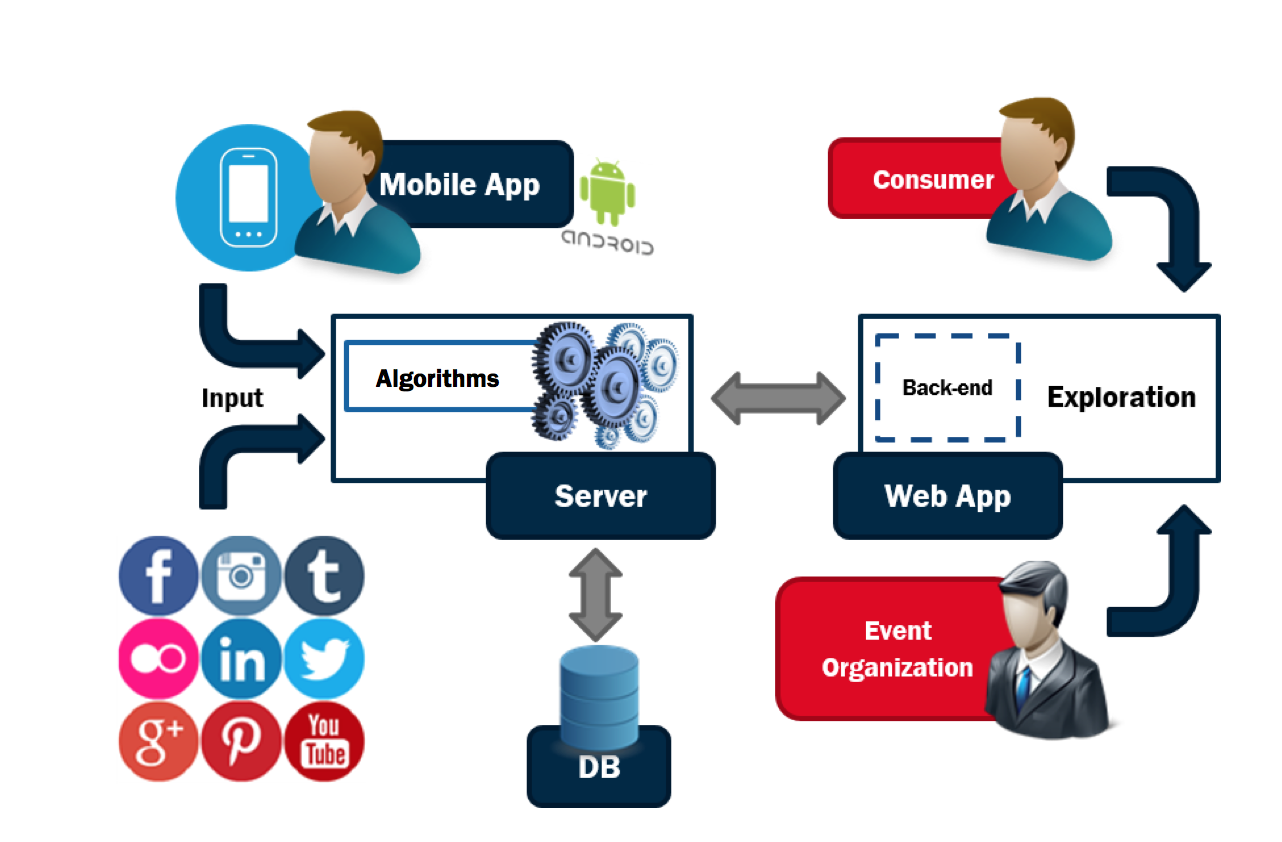
\epsfig{file=architecture.eps, width=2.72in}
	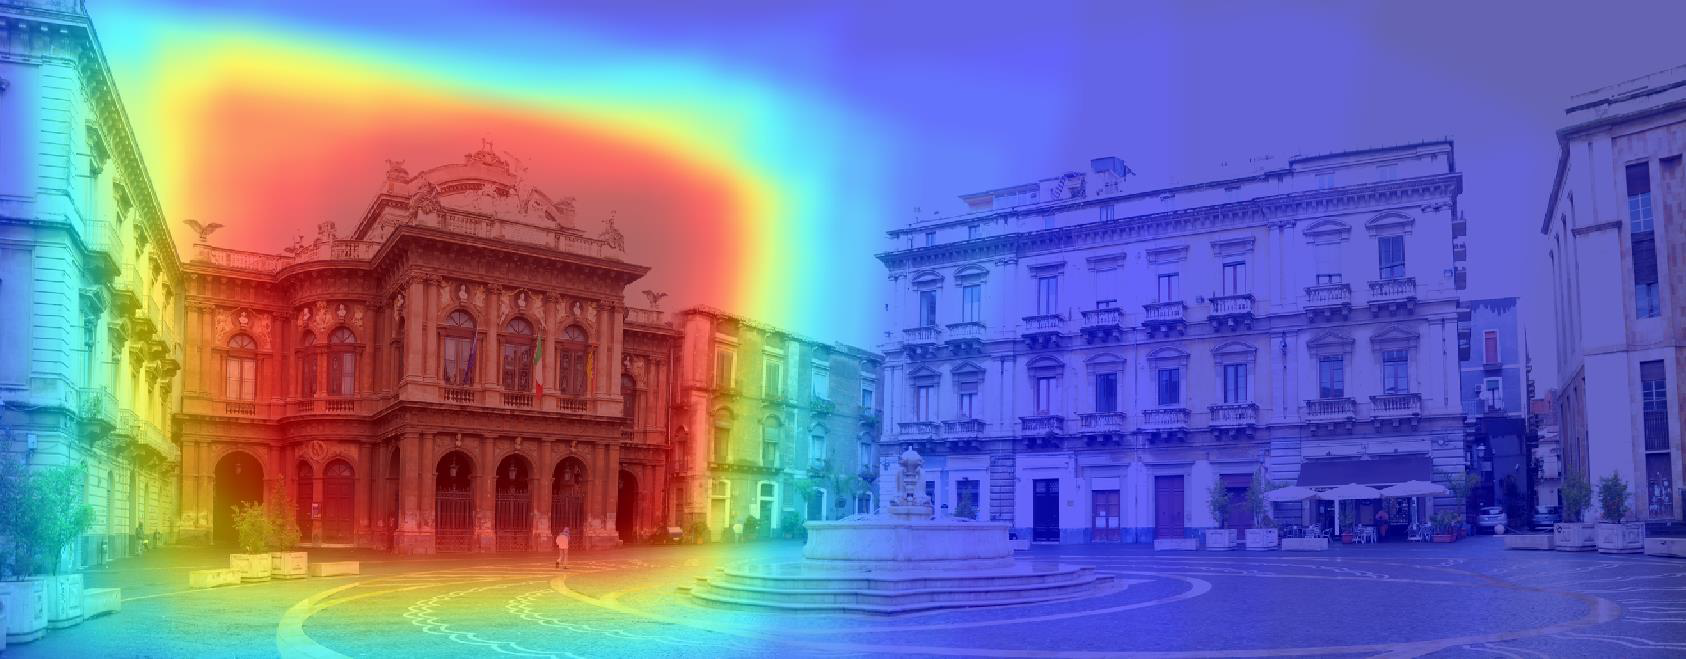
\includegraphics[width=1\linewidth]{heatmap}
	\vspace{-0.7cm}
	\caption{Heat map visualization.}
	\label{heatmap}
\end{figure}

\section{Architecture}
The architecture of the developed framework is shown in Figure \ref{architecture}.
Users can add an image to an event's collection by using a mobile application that gives access to \textit{The Social Picture} repository (TSP). The new images can be uploaded in TSP by using a mobile camera or by selecting images from the most common social networks for images (e.g. Flickr, Panoramio, Instagram).
Once an image is uploaded, it is analysed by a set of Computer Vision and Machine Learning algorithms, and then stored in the database, together with the extracted features and the inferred high level attributes (e.g., type of scene recognized by the algorithm). These information are exploited in TSP to create smart interfaces for the users, which can be used during the exploration of the images related to an event's collection.
The framework collects all the data uploaded by the users of an event, and exploits this crowdsourced multimedia flow of pictures to infer social behavioural information about the event (e.g., by considering the popularity of the uploaded scenes \cite{Ortis2015n525}).

The collections can be explored from smartphones, tablet or desktop computers via a web application, which exhibits a range of filtering tools to better explore the huge amount of data (see Figure \ref{interface}).
%\subsubsection{Database}
%When a new image is added to the system, it is analysed by a set of algorithms with the aim to extract pre-defined features (both visual and textual), as well as semantic information. The image is collected, entered, processed and all the analysis results are stored in the Database.
%\subsubsection{Mobile App}
%The mobile application allows users to upload their visual contributes to the event's collection. Other users can also contribute to the creation of the collection by posting their contents through the considered social netwoks, by adding a specific event's hashtag.
%\subsubsection{Web Application}
The web application shows different interfaces depending on the specific user and the event in which he has joined after an invitation from the event manager (the person who created the event). To join an event's collection, the user must upload at least one picture related to that event. Collections can be explored by several data visualization enviroments, which are selected by the event manager. Anyone registered to \textit{The Social Picture} can become an event manager and start a social collection: this follows the ``prosumer'' paradigm, where the users are both producers and consumers of a service.
The developed framework is characterized by a modular architecture: new visualization interfaces, as well as new semantic filters can be independently created and futher added to the system.
Thus, when an event manager creates a new collection, he is allowed to specify several options to customize the image gathering, the social analysis to be performed, and the visualization tools to be shown for the users of that collection.
The event manager is also allowed to set a range of statistics, which will be available after the analysis of the collected images. These statistics helps organizers to extract useful social information from the crowdsourced pictures \cite{Milotta2016n544}. For example, what is the most popular artwork of a museum? What is the least considered? From which perspective these pictures were taken?
These information could be exploited, for example, to perform aimed investments. The system can suggest what is the better subject to use for the advertising campaign of the event, or which of the attractions it worth to mainly reproduce in the souvenir shop products, to support merchandising strategies. Feedback about what is the most interesting part (i.e., the most photo captured) of a landmark building can help on taking decisions about renovating some parts rather than others as first investment. The connotation of importance is achieved by the crowd who generated ``the social picture'' for that building by uploading related images.
\begin{figure}
	\vspace{-0.3in}
	\centering
	%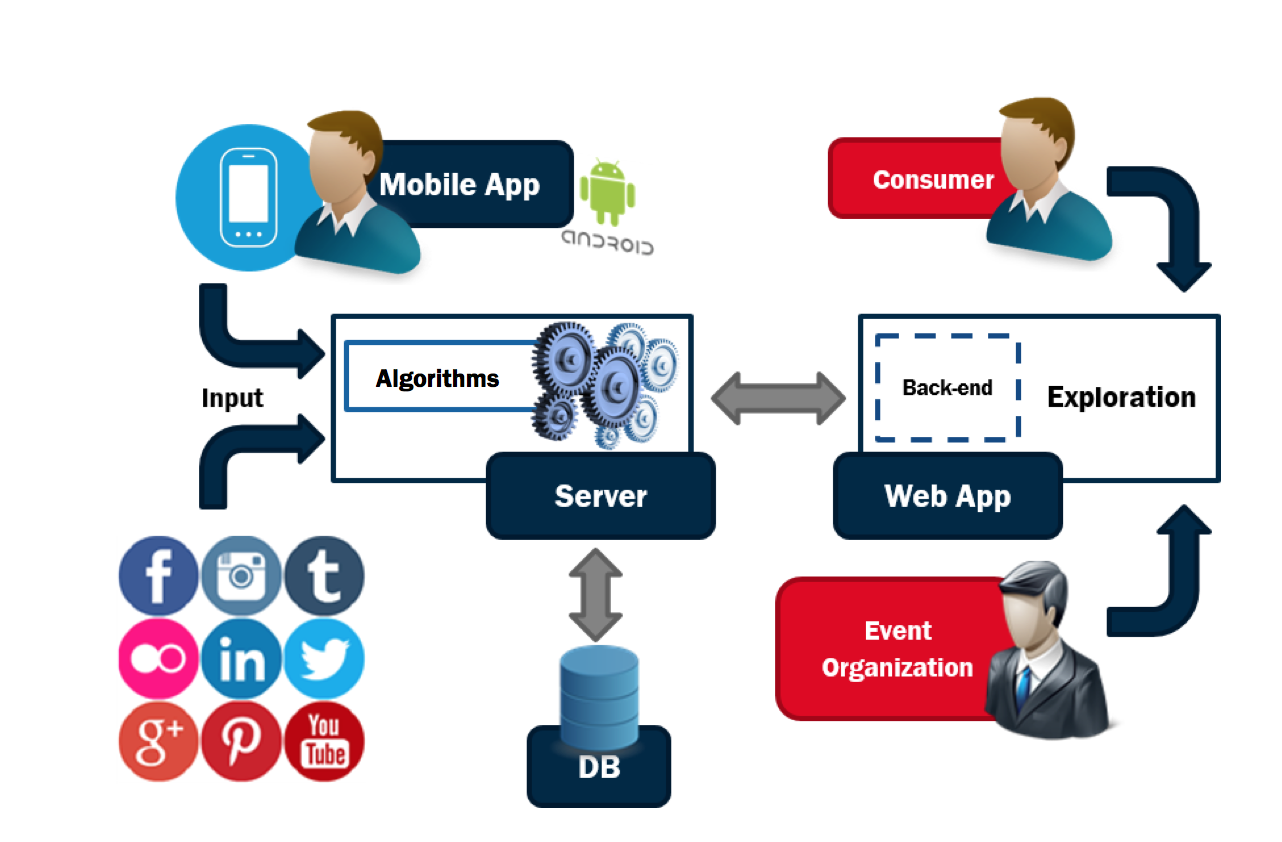
\epsfig{file=architecture.eps, width=2.72in}
	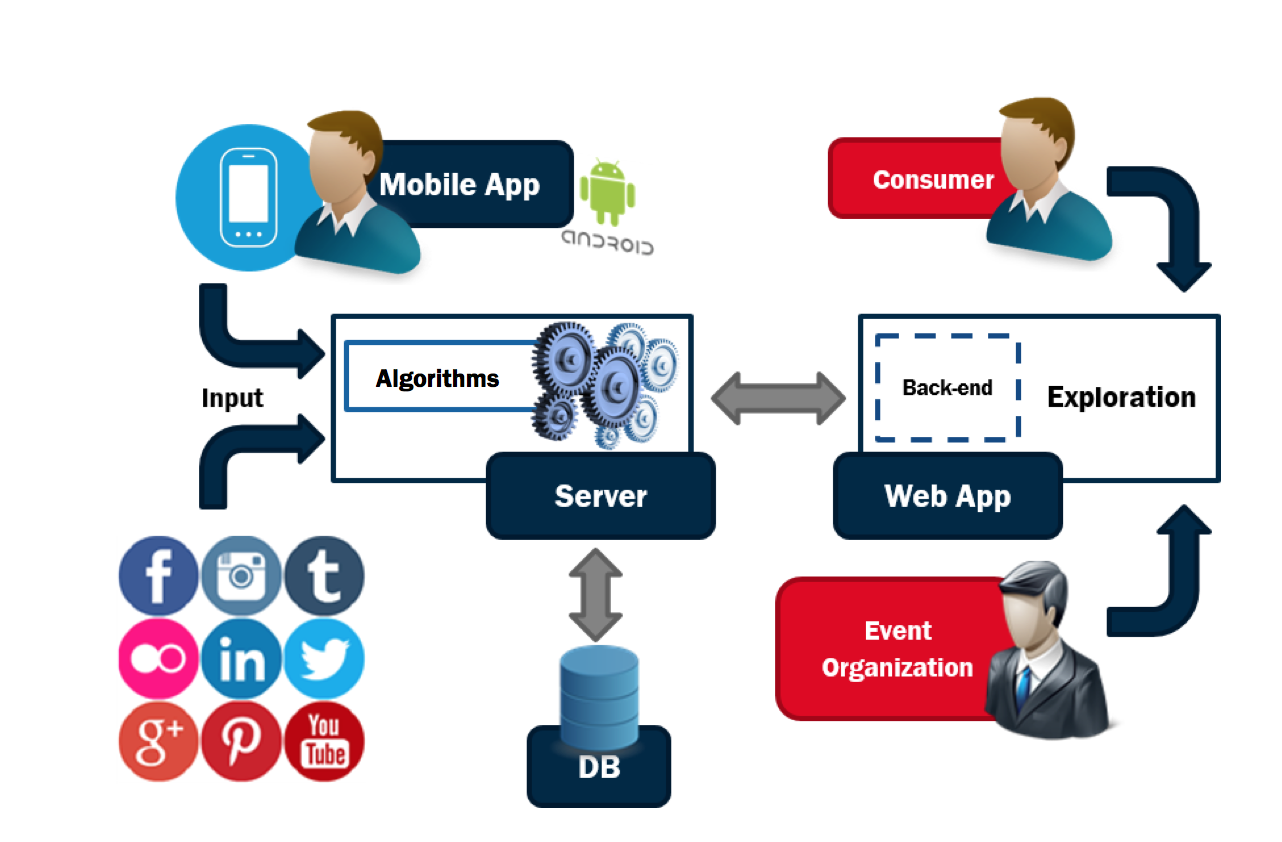
\includegraphics[width=1\linewidth]{architecture}
	\vspace{-0.7cm}
	\caption{The Social Picture's architecture.}
	\label{architecture}
\end{figure}

\begin{figure*}
	\centering
	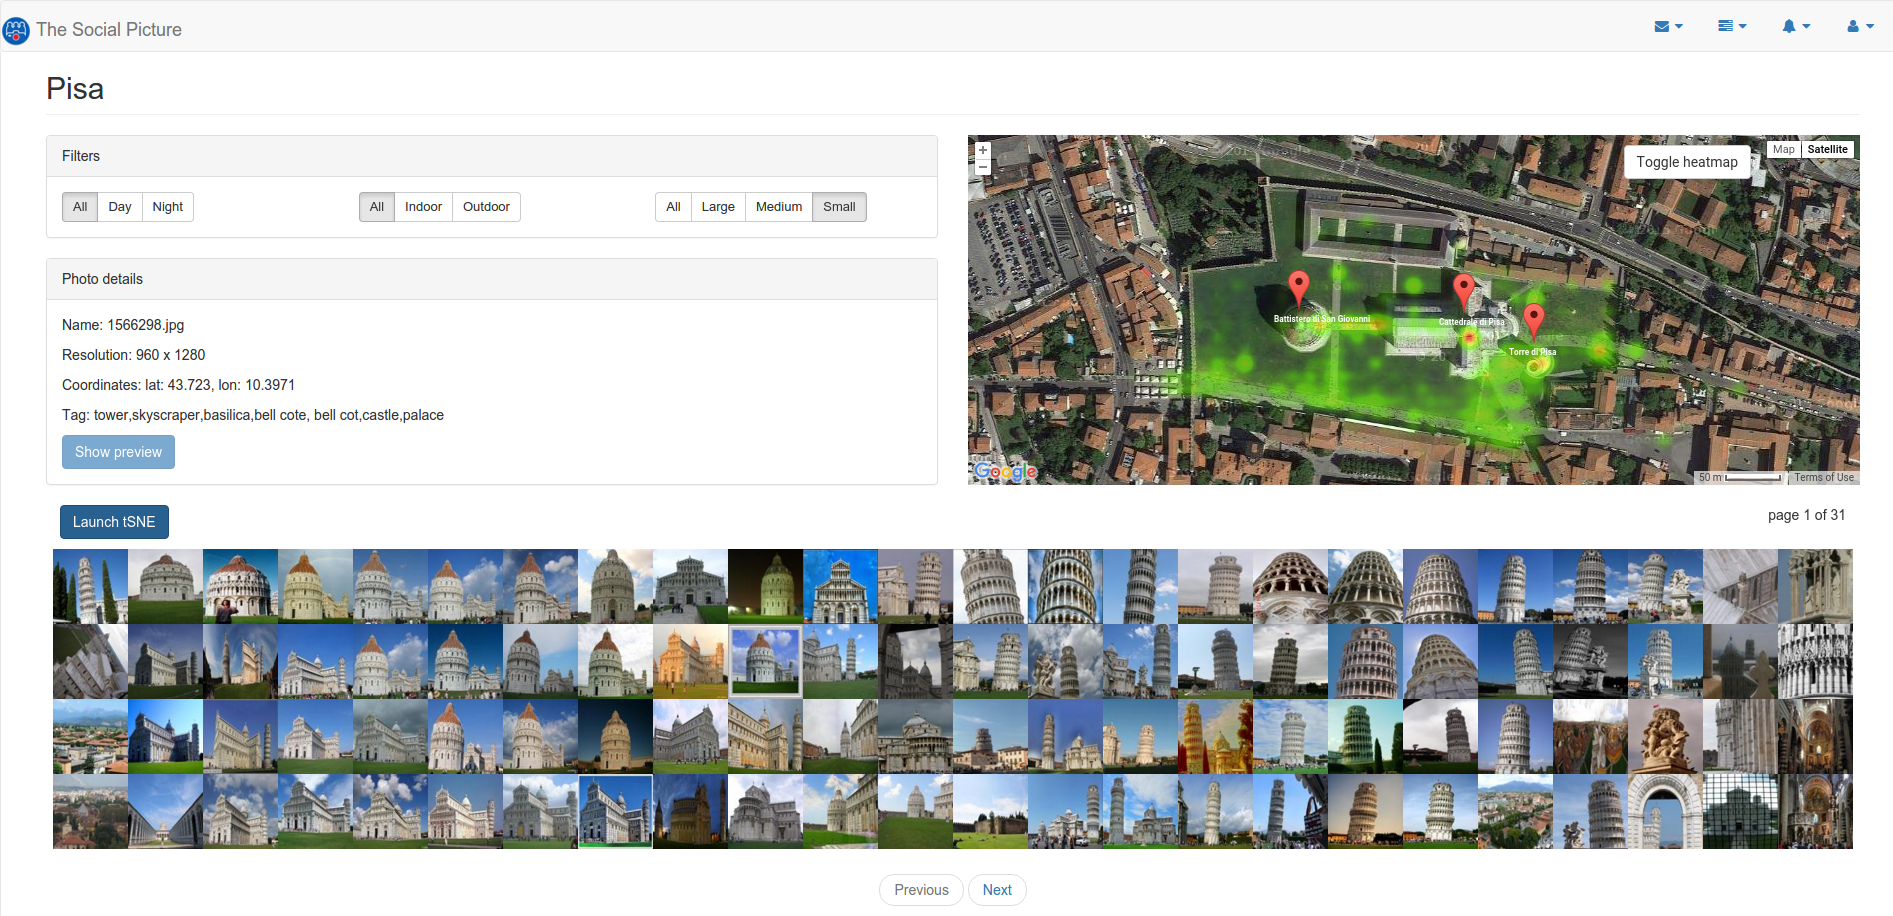
\includegraphics[width=1\linewidth]{interface01}
	\vspace{-0.7cm}
	\caption{Example of exploration interface. It is composed by three main areas: the map area (upper-right) shows the positions where the images have been taken from. This gives the positions of the users during the event and some hints about the most interesting parts of the site. The interaction with this map allows the users to know more details by selecting the images from their positions. The gallery (bottom) shows the  collection organized by using t-SNE algorithm and considering the selected filters. The area upper-left of the interface shows the details of a picture selected from the gallery and presents the available filters.
		From this interface, the user can launch the t-SNE algorithm on a subset of images obtained applying one or more filters, and to know more about the statistics performed by the system on the subset of images.}
	\label{interface}
\end{figure*}

%\subsubsection{Analysis engine}
The several exploration tools are based on both visual and textual data. The system exploits information such as Exif data (camera model, geolocalization, acquisition details, JPEG compression, and others) when available, and a number of ad-hoc extracted visual features.

The visual analysis module of the system feds all the images into two different CNNs \cite{krizhevsky2012imagenet, zhou2014learning}, in order to extract the classification labels and image representations. To attach semantic labels to the visual content of the images, we used \textit{AlexNet}~\cite{krizhevsky2012imagenet} and \textit{Places205-AlexNet}~ \cite{zhou2014learning}.
The CNN used in~\cite{krizhevsky2012imagenet} consists of seven internal layers with a final 1000-way softmax which produces a distribution over the 1000 predefined classes of the ImageNet dataset \cite{ILSVRC15}.We considered the feature activations induced at the last hidden layer, which consists of 4096 dimensional feature (fc-7 feature), as an image representation to be further used with t-SNE algorithm~\cite{van2008visualizing} for visualization purposes.
We also fed the images to the \textit{Places205-AlexNet} CNN \cite{zhou2014learning}. This CNN has the same architecture of \textit{AlexNet} CNN, but it was trained on 205 scene categories related to places learned by using the database \textit{Places205-AlexNet} composed by 2.5 million images.

%The results of the image evaluation by the above CNNs consist of the three classification predictions with the highest scores, given by each CNN, and the fc7 image representation.
\section{User experience}
An event manager (i.e., a user of \textit{The Social Picture} which starts a new collection) creates a new event by selecting among three possible types of event: public event (e.g., a concert), cultural heritage site (e.g., a museum) or private event (e.g., a wedding). The available event categorization can be further extended to include other customized categories. We considered these three categories to better focus the aims of the specific analysis, as well as the inferred information that an organizator wants to extract.
The data gathering from users can be performed within a specific time window. The manager is allowed to control the image acquisition by selecting fine-grained criteria such as filtering media by hashtag, associated text or geolocalization distance.
After creating the event and its acquisition settings, the manager can select the statistics that the system have to compute by exploiting the collection of multimedia data gathered for that event.

The pictures can be grouped by hierarchical categories depending on the combination of two or more of the extracted visual features, this allows us to create several taxonomies in the image collection (panoramic pictures versus close-ups, natural versus artificial, indoor or outdoor, the presence or absence of crowds, selfies versus not selfies, and others).
Specific image categorizations help users to better handle huge amount of crowdsourced pictures, this kind of grouping can be exploited as a pre-processing stage before performing an image based visual search. Given a seed image, the system selects a set of similar pictures.
The system provides different exploration tools. There is a tool for the exploration of outdoor collections such as cultural sites. % and whenever a large environment image can be considered as a reference for more detailed ones,
One more tool can be exploited to better navigate any huge image collection. These exploration tools together with other advanced tools are described in the next subsections.
A video of the demo is available at the following link:
http://iplab.dmi.unict.it/TSP

\subsection{Heat Map Exploration}
In a cultural heritage site, people usually take pictures from different points of view and consider different details and parts related to famous and appreciated attractions and artworks. The heat map exploration tool of \textit{The Social Picture} aims to infer the ``interest'' of people with respect to the different parts of a site. An example of heat map generated from data in \textit{The Social Picture} is shown in Figure \ref{heatmap}. Through this visualization tool, an organizer of a collection will be able to know which parts of the site captures people's interests.
On the other hand, users can explore the collection related to a site in a very simple and intuitive way. So, to highlight the ``interest'' of people related to parts of a site, the proposed system creates an heat map by aligning images in \textit{The Social Picture} with respect to panoramic images of the site of interest \cite{Mikulík2015}.

The heat map is a visualization used to depict the intensity of images at spatial points. The heat map consists of a colored overlay applied to the original image. Areas of higher intensity will be colored red, and areas of lower intensity will appear blue. The intensity of the heat map is related to the number of collected pictures that contain that visual area.
By clicking on a point of the heat map, the user can retrieve and visualize the images that contribuited to generate the map intensity at that point. This set of pictures can be further refined by selecting one of them to ask the system to search similar pictures, or use the image subset as a starting point for furhter analysis. In other words, the heat map visualization gives the possibility to understand the behaviour of the people. Also it can be considered as a powerful and intuitive image retrieval tool for the collections related to cultural heritage sites.


\begin{figure*}
	\centering
	%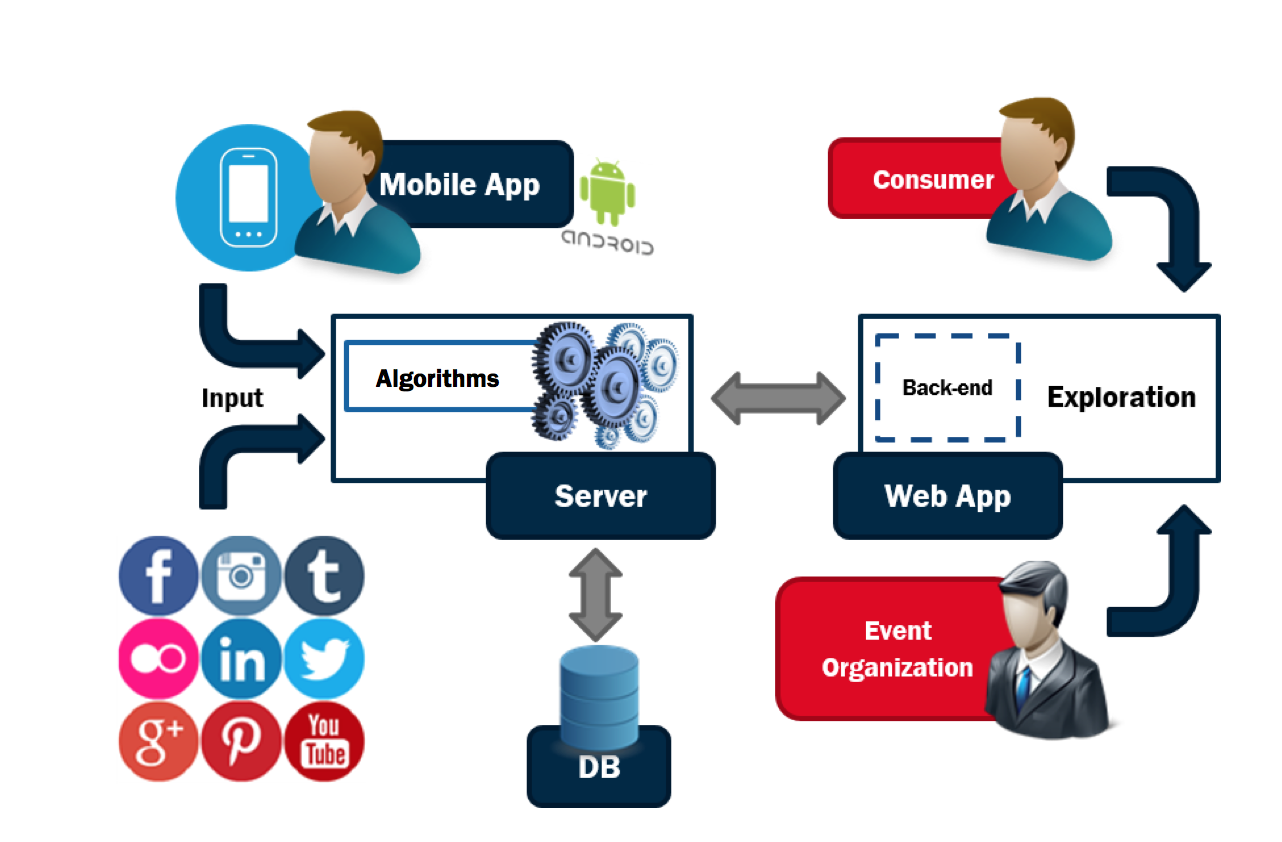
\epsfig{file=architecture.eps, width=2.72in}
	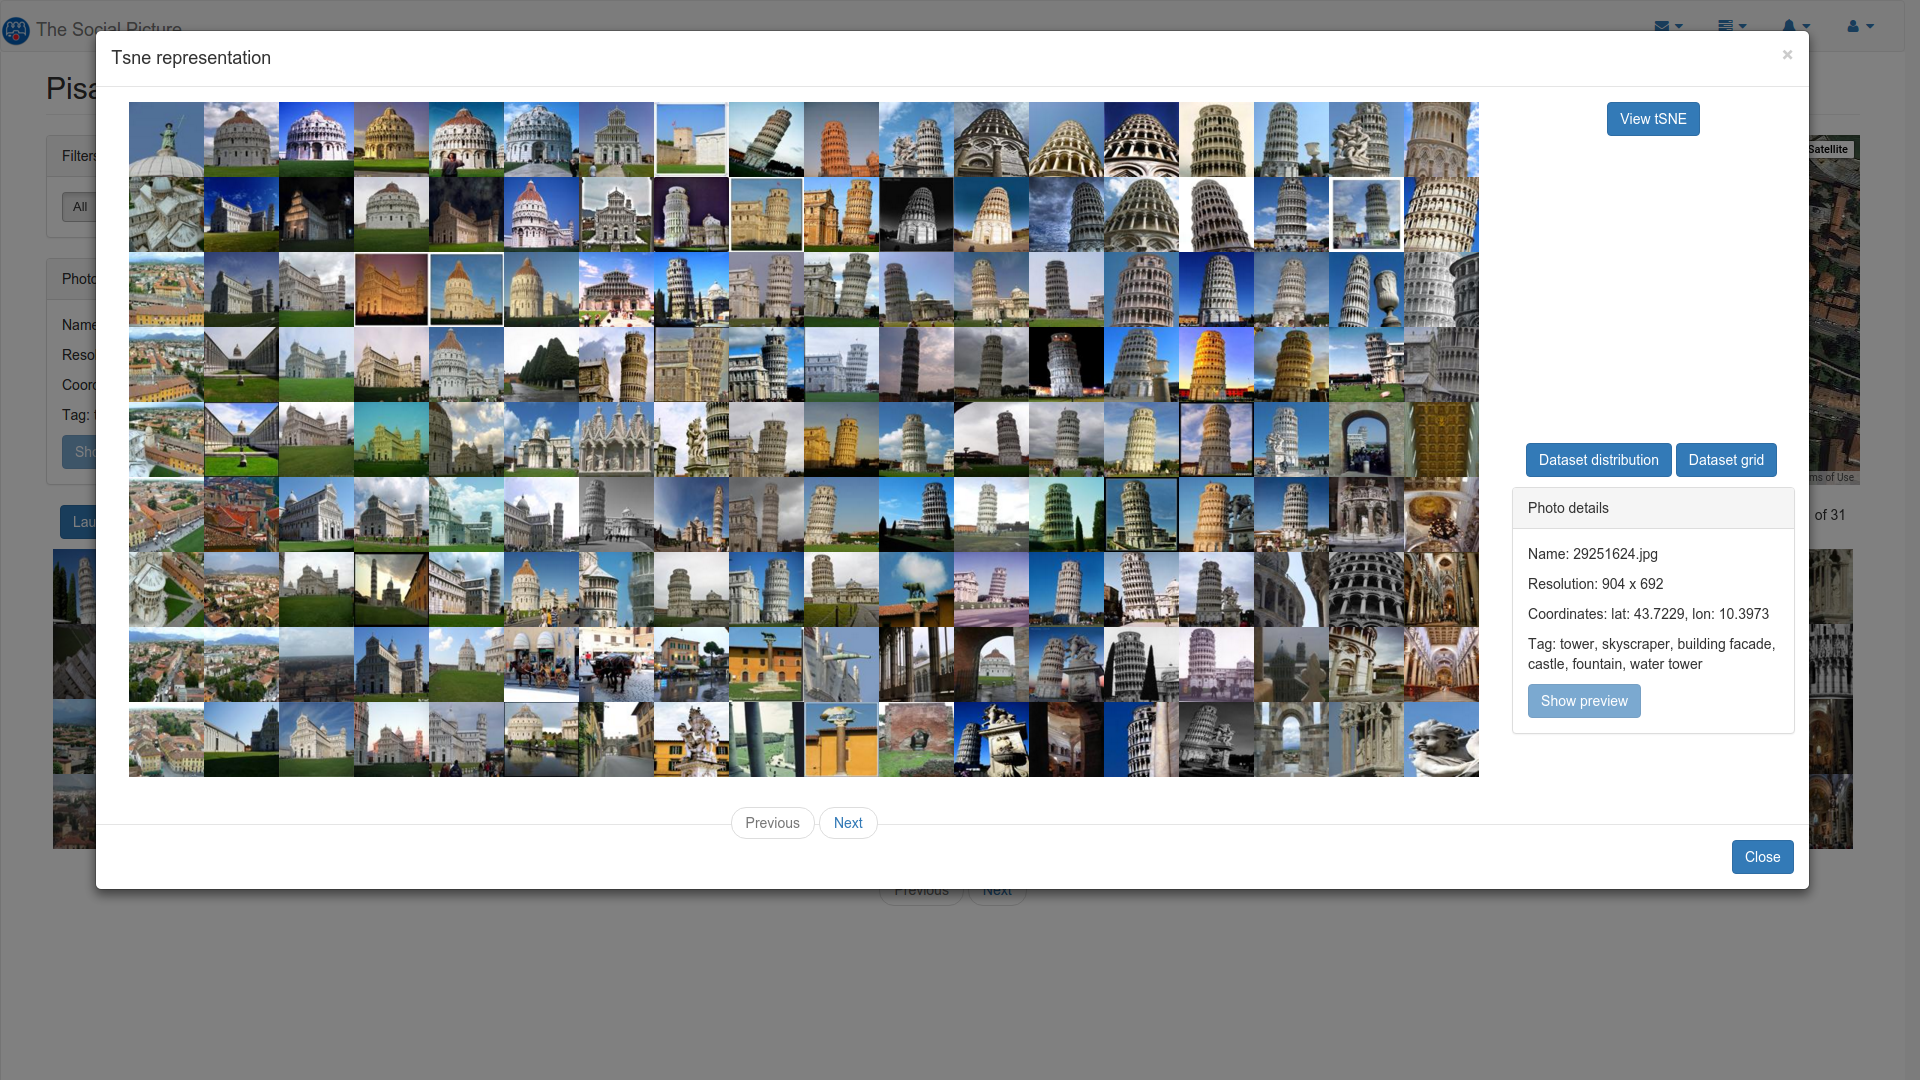
\includegraphics[width=1\linewidth]{gridtsne}
	\vspace{-0.3cm}
	\caption{t-SNE visualization. The images are forced to fit a grid layout. Images of an event are automatically organized by visual content. Images close in the 2D layout are also close in terms of visual content.}
	\label{gridtsne}
\end{figure*}
\subsubsection{3D Reconstruction}
Starting from VSFM (Visual Structure From Motion)~\cite{wu2013towards}, we are able to compute a 3D sparse reconstruction of large photos collections. The models are augmented with colors for vertices, related to the frequency of been acquired in a photo, colors for cameras, related to the number of visual features acquired by each photo, and with a plane which show the spatial density of contributing users. We embedded in TSP the models through a 3D web viewer based on Threejs, allowing the users to browse the 3D sparse reconstructed models gaining a cue about what are the points of view and the subjects preferred by users when take photos. Moreover, the models in the 3D web viewer can also be browsed through Leap Motion system, an intuitive and fast interactive system.
\vspace{-0.2cm}


\subsection{t-SNE Exploration}
We exploit the fc7 feature extracted with the \textit{AlexNet} architecture \cite{krizhevsky2012imagenet} for each image and use the t-SNE embedding algorithm \cite{van2008visualizing} to compute a 2D embedding that respects the pairwise distances between visual features, forcing to fit a grid layout (Figure \ref{gridtsne}). The t-SNE (t-Distribuited Stochastic Neighbour Embedding) is a technique for feature space dimensionality reduction that is particularly well suited for the visualization of high dimensional image datasets.
Note that images with the same subject are automatically arranged nearby (see Figure \ref{gridtsne}). Moreover, the system arranges very close those images which are not the same but have a similar visual content. It is also important to highlight that the employed CNN \cite{krizhevsky2012imagenet} has been trained using a different dataset concerning 1000 classes of objects, but the fc7 features resulted expressive and representative enough to be applied succesfully to a generic event collection.

%Another exploration tool, allow users to see the result of t-SNE embedding without using the grid layout. If we display a set of images using their embedded locations computed by t-SNE, they may overlap one each other. Especially if there are many similar images. For this reason, this interface provides a set of tools to help the user's navigation.

With this exploration tool, the user can apply a translation or a zooming to all the viewed images, just clicking and dragging the mouse along the desidered direction and by using the scroll wheel respectively. This helps the user to better explore the image distribution in a custom level of detail.
%A number of tools enable users to fine-tune the spread of images along X and Y axis, and the zooming effect. These parameters can be used to transform the distribution of the embedded images, and adapt the effect of the mouse commands. For example, if the user fix an upper bound for the zoom effect, when this limit is reached the scrool wheel of the mouse has the effect of separating the images according to the amout of the rotation.
Furthermore, the user can choose a subset of images and compute the t-SNE embedding of them directly on the browser (see Figure \ref{gridtsne}).% This tool has been developed by using the \textit{tsnejs} Javascript library by Andrej Karpathy.
\subsubsection{Hierarchical t-SNE}
The first implementation of the t-SNE exploration tool in TSP was unable to scale with the number of the collections' images. The new tool presented in this demo implements an hierarchical version of the t-SNE embedding which allows to explore picture collections without limits on the amount of processed pictures. 
This helps the user to better explore the image distribution in a custom level of detail. Furthermore, the user can choose a subset of images and compute the t-SNE embedding of them directly on the browser. % This tool has been developed by using the \textit{tsnejs} Javascript library by Andrej Karpathy.
As the number of pictures of a collection is unpredictable, the computation of the t-SNE coordinates could be very expensive. Besides the t-SNE computation, which needs to be executed only one time per dataset, a huge number of pictures can affect the browser efficiency for the visualization of the 2D embedding. We organize the entire collection of pictures in a hierarchical structure. After the collection is analysed (i.e., the \textit{fc7} features have been computed for all the images) the system performs a hierarchical k-means clustering of the image features. The algorithm divides the dataset recursively into \textit{k} clusters, for each computation the \textit{k} centroids are used as elements of a \textit{k-tree} and removed from the set. %Each node has \textit{k} children nodes (even empty), each one containing the cluster elements associated to the corresponding centroid. Since each node cannot contain more then \textit{k} elements, when this number is higher than \textit{k} the clustering is repeated recursively. 
When this new version of the t-SNE tool (hierarchical t-SNE) is executed, it shows to the user the t-SNE embedding computed only for the elements in the root of the \textit{k-tree} (i.e., the picture centroids of the first \textit{k-means} computation). When the user selects one of these pictures, the system computes the t-SNE of the pictures included in the child node corresponding to the selected picture element. This hierarchical exploration can be continued by selecting one of the shown pictures and computing the t-SNE embedding for its sub-elements in the hierarchy.



\subsection{Other Advanced Tools}
%\begin{itemize}
%	\item Subsampling from set of images
%	\item Captioning-Image Description:
%	with the aim to obtain better image descriptions, the system can generate a set of captions associated to each image. The dense captioning task generalizes object detection when the descriptions consist of a single word, and Image Captioning when one predicted region covers the full image \cite{Johnson2015densecap}. The result of dense captioning can be exploited to provide a description based image retrieval system, and an image description with an higher level of abstracton compared to the one given by an image classification approach.
%	\item Questions and Answers for assistive:
%	in the last few years, with the improvements in both natural language and image understanding, much effort has been spent by scientific community to develop algorithms for question answering on real-world images \cite{VQA}. These systems take and image and a natural language question about the image content, and provide a natural language answer. Such a system can be easily integrated in the \textit{The Social Picture} platform with the aim to improve its interfaces, allowing the visually impaired to know about the image collection's visual contents. The user is allowed to ask natural language questions about single images, the entire collections or an its subset.
%\end{itemize}
%
Among the tools included in \textit{The Social Picture}, there is the one useful to generate automatic subsets of images from a specific photo collection. This tool allows the user to set the number of images to obtain as output for a collection in TSP, and automatically generates the subset of images taking into account visual features as well as EXIF information related to the images composing the photo collection (e.g., GPS location, TAGS, day, time, etc). In this way, the user can have some representative image prototypes related to the collection to be used for different purposes (e.g., printing the most significant pictures of paintings of a museum for a specific social group). For this tool CNN representation used in~\cite{zhou2014learning} is employed.

One more feature included in The Social Picture is the automatic image captioning, as described in \cite{karpathy2015deep}. With the aim to help the user to include a description to an uploaded image, \textit{The Social Picture} automatically generates and suggests a description to the user that can then refine it.  The descriptions of images can be used for text based query performed by the user.


\section{Image Polarity Prediction}

\section{Image Popularity Prediction}

\section{Conclusions}